\begin{itemize}
\item Introduction for the implementation section.
\item Introduction should perhaps introduce the topics of this chapter.
\end{itemize}

\section{Methodology}
\label{sec:methodology}
Methodology here.

\textbf{What is the implementation chapter about?}\\
This chapter delves into the development of several prototypes, each portraying different types of behaviour for hands in VR. These different prototypes have similarities and differences in their approach to the problem. In the following sections we will present a categorization of approaches that can be taken when implementing hands in VR, what effect these different approaches have and their pros and cons.

\textbf{What stuff did we use during the project?} (headset and control scheme, for instance)\\
The prototypes have all been developed using the Unity engine which means that to their implementations are restricted by the API that Unity provides. Furthermore, during development and testing, we’ve been using the HTC Vive and its default controllers as the input method for the hands.

Since we have been using the HTC Vive and its default controllers as input to control the hands our approaches are more applicable to hardware that has the same affordances as these controllers. We use the position and orientation input from the controllers to position and rotate the hands in the virtual space and we use the trigger button to indicate how much the fingers should bend or how closed the hand should be.

\todo[inline]{Mention the use of Unity as well.}

\textbf{How does this lead into the categorizations?}\\
These three inputs are the base of the categorizations of approaches. Each of these inputs can be filtered, by which is meant that the input can be modified or skipped. Filtering on one of the inputs can be seen as using that input as the parameter for a function, which returns a new result. A hand can have a filter for either none of the inputs or one of the inputs or more. Different filtering combinations will give a different behaviour for the hand in the virtual world and might result in the hand seeming more realistic when interacting with its environment.

\todo[inline]{Maybe structure this chapter so that the different hand prototypes are introduced with their name before going into the specific filtering sections (for instance position filtering). Then inside the filtering sections the hands can be mentioned with their differences. After all the filter sections there can then perhaps be a section that reiterates over the hand prototypes and summarises their filtering implementations.}

\section{Categorization of approaches}
\label{sec:categorizationOfApproaches}
\begin{itemize}
\item Lead into the explanation for the filter variables.
\item Display filter variable table.
\item Describe several examples of filter variable combinations and show image sequences.
\item (Describe the reasons and effects for filtering on the different variables)?
\end{itemize}

The three player inputs mentioned above (position, orientation and how closed the hand should be) are the base of the categorization of approaches. Each of these inputs can be filtered, by which is meant that the input can be modified or skipped. Filtering on one of the inputs can be seen as using the input as the parameter for a function, which returns a new result which will be used instead of that input. A hand can be implemented with filters on several inputs at once and can have different filters depending on the context. Different filterer combinations will give a different behaviour for the hand in the virtual world and can result in the hand seeming more realistic when interacting with its environment.

\begin{table}[H]
\centering
\caption{Filter variable combinations.}
\label{tab:filterVariableCombinations}
\begin{tabular}{C{2cm}C{2cm}C{2cm}}
Position & Rotation & Finger position \\ \midrule \midrule
				&					&					\\ \midrule
\Large X	&					&					\\ \midrule
				& \Large X	& 		                \\ \midrule
				&					& \Large X     \\ \midrule
\Large X	& \Large X	&					\\ \midrule
\Large X 	&					& \Large X	\\ \midrule
				& \Large X	& \Large X	\\ \midrule
\Large X 	& \Large X 	& \Large X
\end{tabular}
\end{table}

\subsection{Position filtering}
\label{subsec:categoryPositionFiltering}
\textbf{Questions to answer in this section:}
\begin{itemize}
\item What does it mean to filter the player's positional input?
\item Why do we want to filter the player's positional input?
\end{itemize}

\textbf{What does it mean to filter the player's positional input?}\\
A position filter using the definition above is a function, which when enabled, takes the player's positional input from a controller and returns a new value to be used in its stead. This means that the position of the hand in the virtual world will deviate from the controller position.

\textbf{Why do we want to filter the player's positional input?}\\
One of our hypotheses is that it's possible to increase the player's sense of embodiment by simulating more realistic behaviour for hands around objects in the world. One of the first steps here is to not allow the hands to penetrate objects. By using position filtering to deviate the hand from the controller position when trying to penetrate an object, the hand can interact more realistically with the world.

The following two figures show an image sequence of a hand with no input filtering and an image sequence with a hand that uses position filtering. The second figure shows that the hand is stopping when it reaches the object, whereas in the first figure the hand moves through the object.

\begin{figure}[H]
\label{fig:filtersNone}
\centering
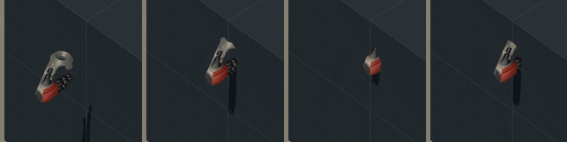
\includegraphics[width=\textwidth]{Sequences/FiltersNone/Seq_FiltersNone.png}
\caption{Sequence showing hand without filters entering obstacle.}
\end{figure}

\begin{figure}[H]
\label{fig:filtersPosition}
\centering
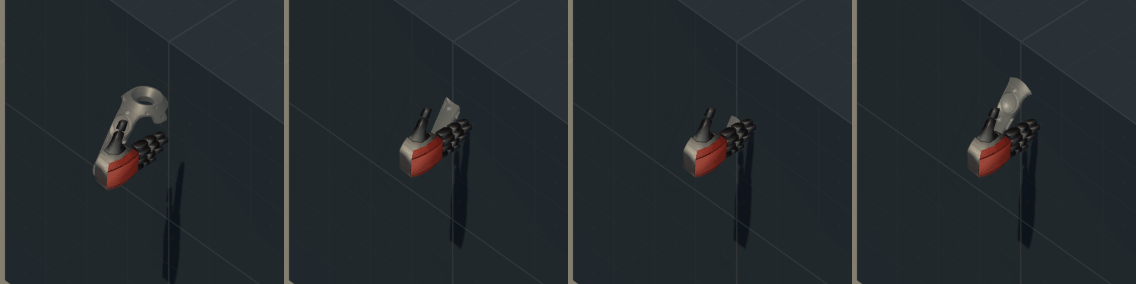
\includegraphics[width=\textwidth]{Sequences/FiltersPosition/Seq_FiltersPosition.png}
\caption{Sequence showing hand filtering on position. Notice the controller continuing to move into the obstacle.}
\end{figure}

\textbf{Questions to answer in this section:}
\begin{itemize}
\item How can we filter the player's positional input?
\begin{itemize}
\item Depenetration.
\item Physics system.
\item Different filter methods have different restrictions.
\end{itemize}
\end{itemize}

\textbf{How can we filter the player's positional input?}\\
The position filters we have implemented can be split into two distinct categories: a pre-collision correction category and a post-collision correction category. Using a pre-collision correction method in the case of disallowing the penetration of objects means to never allow the hand to enter an object by anticipating the penetration in advance. Using a post-collision correction method in the same case means to correct the hand's position after the collision has happened.

Position filtering in the case of disallowing the penetration of objects can be implemented in several ways. One of the methods used during this thesis project is to detect a collision between the hand and an object in the world and take action when such a collision occurs. The manual collision checking can be implemented by checking for nearby object colliders and using ray casts or sweeps to anticipate the collision.

Another implementation uses the physics system to handle collisions between the hands and obstacles in the world. The hands are moved by setting their velocities in such a way that they would reach their target within the current frame.

\subsection{Rotation filtering}
\label{subsec:categoryRotationFiltering}
\textbf{Questions to answer in this section:}
\todo{Alternative term: orientation}
\begin{itemize}
\item What does it mean to filter the player's rotational input?
\item Why do we want to filter the player's rotational input?
\begin{itemize}
\item Reduce position filtering.
\item Display player's intentions.
\item Diagetically communicate available interactions.
\item Allows for more detailed hand animation depending on available interactions. Control?
\item Mention stiffness with only position filtering
\end{itemize}
\end{itemize}

\textbf{What does it mean to filter the player's rotational input?}\\
To use a rotation filter is to deviate the hands rotation from the current orientation of the controller. In certain contexts it can be beneficial filter on rotation on order for the hand to seem more alive and realistic. Hands can adapt their rotation in several ways and different approaches might be taken depending on the context. When approaching a wall with their hand a player's intention in the real world might be to place their hand flat on the wall (palm-first). This behaviour can be implemented using a rotation filter, which takes effect when the hand is approaching a surface.


\todo[inline]{Adjusting might be a better word?} Filtering on the rotation input means to rotate the hand differently in the virtual world compared to the rotation of the controller.

\textbf{Why do we want to filter the player's rotational input?}\\
Rotation filtering can be used to display what is assumed to be the player's intention when they interact with the world. One example could be the intention of the player when they approach a wall with their hand. In this case a reasonable assumption would be that the player's intention is to rotate the hand so that the palm faces the wall (See image sequences below). Besides being useful when wanting to adapt the hand to the player's intentions, rotation filtering can also be used in order to reduce the amount of position filtering needed. This means that rotating the hand will allow the distance between the hand and the controller due to position adjusting to be reduced (See image sequence below).

\todo[inline]{use refs}
The first of the two figures below shows an image sequence of a hand using only rotation filtering and the second figure shows an image sequence of a hand using both position and rotation filtering where the rotation filtering is implemented as palm-first towards the surface.

\missingfigure[figwidth=15cm]{Image sequence: Rotation filtering}
\missingfigure[figwidth=15cm]{Image sequence: Position and rotation filtering}

\textbf{Questions to answer in this section:}
\begin{itemize}
\item How can we filter the player's rotational input?
\begin{itemize}
\item Manual rotation filtering when approaching obstacles.
\item Differentiation between object types and angles of approach.
\item Physics system.
\end{itemize}
\end{itemize}

\todo[inline]{Remember explicit vs implicit rotation filtering (explicit being where we completely control the rotation vs the for instance the physics system controlling it).}

\textbf{How can we filter the player's rotational input?}\\
Although all our hands use position filtering, only 2 of our 5 hand prototypes (rigid hands, sliding rigid hands, finger rigid hands, physics hands and advanced hands) use rotation filtering.

For the physics hands, we don't use any explicit rotation filtering. The physics system decides the rotation of the hand, when interacting with surfaces. While the controller is within an object, the physics hand can decide to rotate the hand to a flat position (either palm-up or palm-down) in order to reduce the position deviation between the hand and the controller. The rotation happens as a jump and not as a smooth movement towards the surface resulting in a less natural feel during the jump, but a somewhat realistic look afterwards. To improve upon this, explicit rotation filtering could have been added to smoothly rotate the hand to lay flat on the surface, which could remove the jump altogether, but at the same time introduce complexity to the implementation.

Contrary to the physics hands the advanced hands do use explicit rotation filtering. The goal of the rotation filtering for this hand was to always approach a surface palm-first. The main example to explain this choice is the approach of a hand towards a wall. When a player wants to put their hand on a wall, which way would they want to do this? Having an open hand and moving the hand fingers first wouldn't make much sense. It would not give support if the reason for touching the wall was to lean against it, for instance. Rotating the hand so that the palm would be placed firmly on the surface of the wall would make more sense in this case. With this as the main idea behind the rotation, the implementation then had to support this in several cases. The easy case is when the player approaches the wall with an open hand and the palm being closer to the surface than the back of the hand. Depending on the distance to the surface we rotate the palm of the hand the rest of the way until it is directly facing the surface. Another case is what to do when the hand is closed into a fist. In this case, the player is probably trying to punch the wall, which means that the palm shouldn't be facing the wall. Testing for this case isn't necessarily hard in itself, but other cases pile on top of this, including what to do when approaching with the back of the hand, what to do when the player is rotating while the hand is touching the surface and more.

\subsection{Finger position filtering}
\label{subsec:categoryFingerFiltering}
\textbf{Questions to answer in this section:}
\begin{itemize}
\item What does it mean to filter the player's finger position input?
\item Why do we want to filter the player's finger position input?
\begin{itemize}
\item Reduce position filtering.
\item Display player's intention.
\end{itemize}
\end{itemize}

\textbf{What does it mean to filter the player's finger position input?}\\
Filtering the finger positions is about placing the finger tips in space relatively to the rest of the hand or put differently; stretching and bending the fingers. The fingers can be filtered as a group or individually and different contexts can determine different filters.

\textbf{Why do we want to filter the player's finger position input?}\\
Here, like with the rotation filtering, a certain amount of assumptions have to be made about what the player's intend is. When a player's hand is approaching an object that can be grabbed, the most common case might be that they are trying to grab the object. If this is the case, adjusting the fingers to form a grip could be a natural behaviour.

\missingfigure[figwidth=15cm]{Image sequence: Position and finger position filtering}

\textbf{Questions to answer in this section:}
\begin{itemize}
\item How can we filter the player's finger position input?
\begin{itemize}
\item Filtering to avoid obstacles.
\item Filtering to anticipate player intent.
\item Differentiation between object types and angles of approach.
\end{itemize}
\end{itemize}

\textbf{How can we filter the player's finger position input?}\\
Implementations of finger position filtering include using an animation system to animate the fingers together or individually to different poses and the use of an Inverse Kinematics (IK) system to infer finger pose from finger tip position and hand position and orientation.

\todo{Obviously you skipped the actual methods?}

\section{Description of how we evaluated hand iterations ...}
\label{sec:DESCRIPTIONOFEVALUATIONSCENARIOS}
\todo[inline]{should this be methodology?}

\section{Hands and their filterings}
\label{sec:LABELABOUTHANDSVERSIONS}
\begin{itemize}
\item Describe each hand and what filtering variables they use.
\item Relate hands to the above filtering variable descriptions.
\end{itemize}

\todo[inline]{Decide on which hand prototypes to include in the paper and what to name them.}
\todo[inline]{Add a chart here or to the appendix about all the included hand prototypes and which filters they use.}

\section{Miscellaneous shitz}
\label{sec:MISCELLANEOUSSHITZ}

\subsection{Hand visualization}
\label{subsec:handVisualization}

\subsection{Rumblez!}
\label{subsec:RUMLBEZ}

\subsection{Grabbing system details}
\label{subsec:grabbingSystem}